 \thispagestyle{gocconone}
\pagestyle{gocco}
\everymath{\color{gocco}}
\graphicspath{{../gocco/pic/}}
\blfootnote{$^1${\color[named]{gocco}Đại kiện tướng quốc tế.}}
\begingroup
\AddToShipoutPicture*{\put(0,616){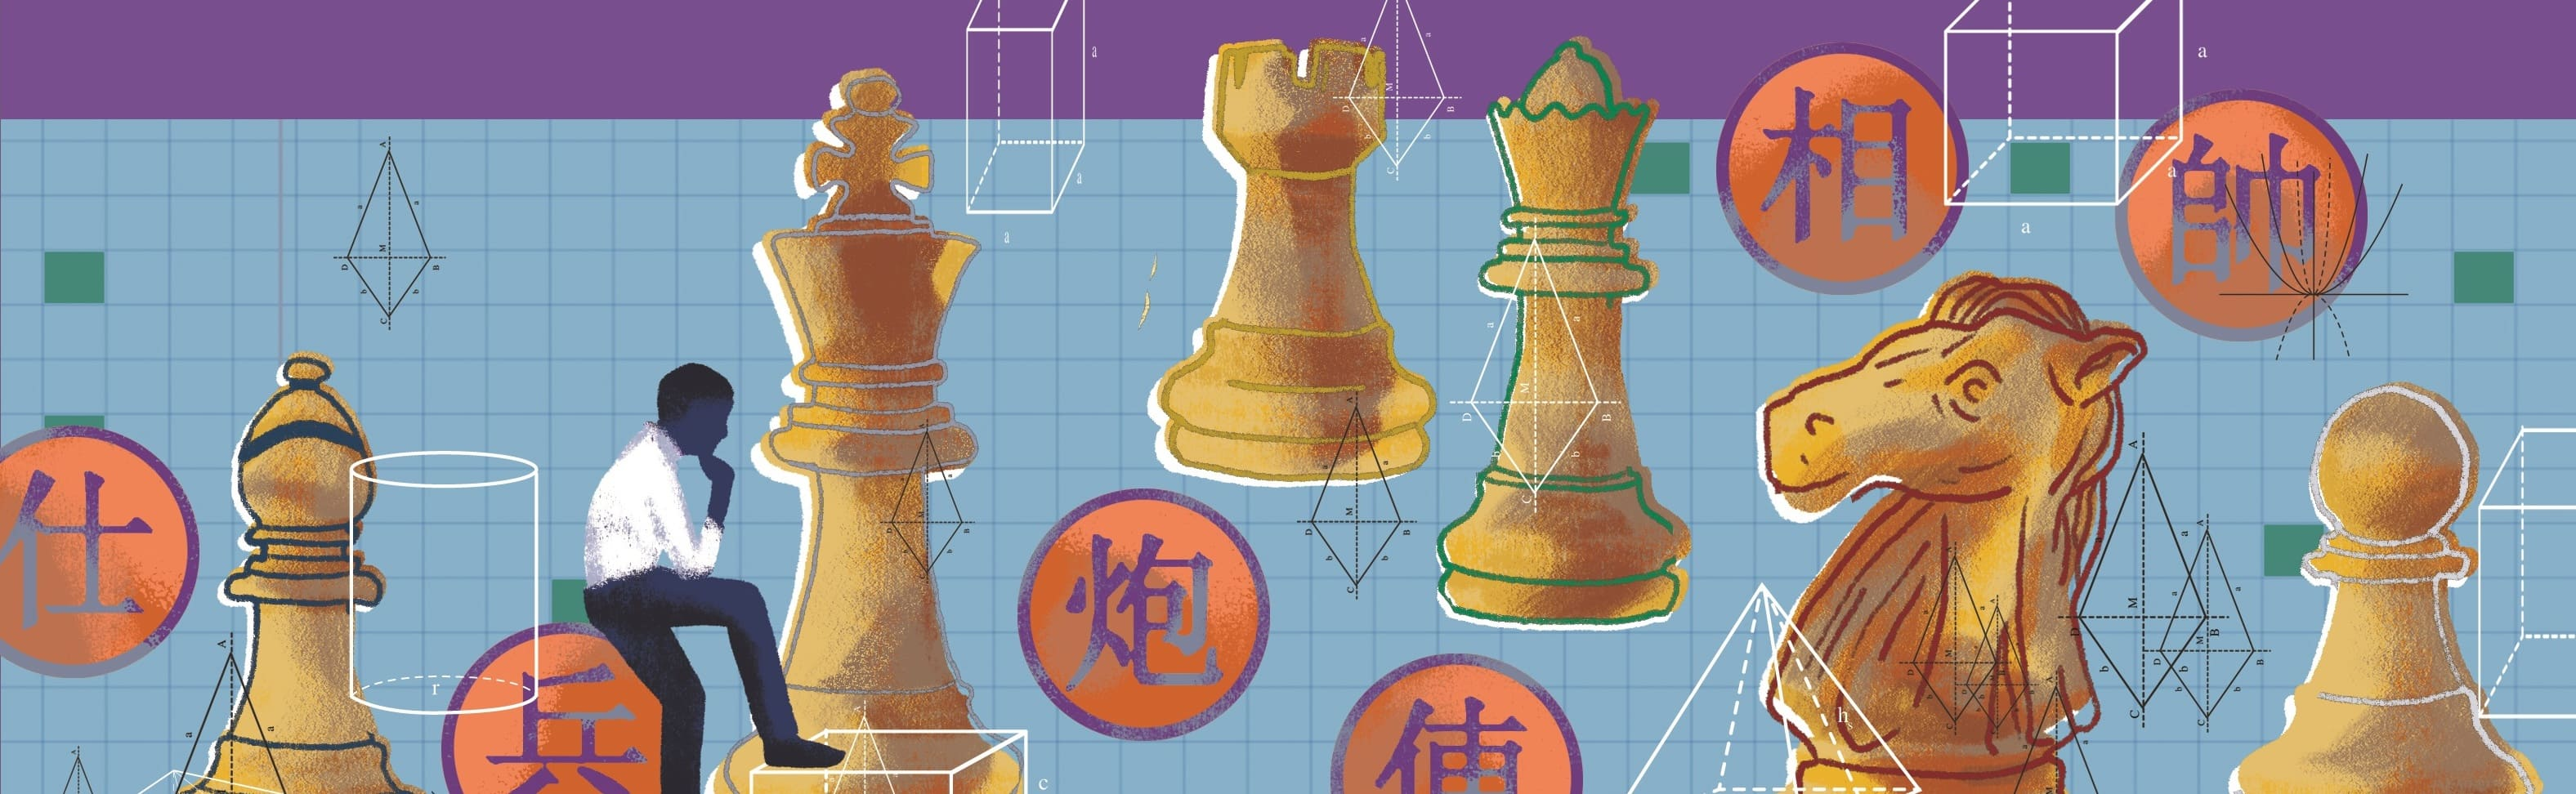
\includegraphics[width=19.3cm]{../bannergocco}}}
\AddToShipoutPicture*{\put(58,552){
\includegraphics[scale=1]{../tieude3.pdf}}} 
\centering
\endgroup

\vspace*{155pt}

\begin{multicols}{2}
	$2.$ \textit{Hậu chống tượng và mã}
	\vskip 0.1cm 
	Hậu chống tượng và mã tương đối đơn giản hơn chống hai tượng. Cơ hội giành chiến thắng của bên có Hậu khá lớn, hơn $98\%$ các tình huống bên có Hậu sẽ xử lý ưu thế thành công.
	\vskip 0.1cm
	Chúng ta xem xét một vài ví dụ sau:
	\vskip 0.1cm
	Ví dụ $1$: NN
	\begin{center}
		\newgame
		\fenboard{8/8/5kn1/5b2/3K4/8/7Q/8 b Q - 0 1}
		\showboard
		\vskip 0.1cm
		\textit{\small\color{gocco}Hình $1$.}
	\end{center}
	Kế hoạch giành chiến thắng của Trắng là kiểm soát các ô mầu đen, mầu ô chỉ mã đen có thể kiểm soát.
	\vskip 0.1cm
	$\pmb{1.}$\textbf{\color{gocco}Hd$\pmb{6}$+ Vg}$\pmb{5}$ [Nếu $1$...Te$6$ $2.$Ve$4$ Vf$7$ $3.$Hd$4$ Tc$8$ $4.$Hf$2+$ Vg$7$ $5.$Vd$5$ Vh$6$ $6.$Vd$6$ Tg$4$ $7.$Hc$5$ Vh$7$ $8.$Hg$5$ Tc$8$ $9.$Hh$5+$ Vg$7$ $10.$Hc$5$ 
	\begin{center}
		\newgame
		\fenboard{2b5/6k1/3K2n1/2Q5/8/8/8/8 b Q - 0 1}
		\showboard
		\vskip 0.1cm
		\textit{\small\color{gocco}Hình $2$.}
	\end{center}
	Đen buộc phải di chuyển mã $10$...Tb$7$ ($10$\textit{...Ta$6$ $11.$Ha$7+$; $10$...Tg$4$ $11.$Hd$4+$; $10$...Th$3$ $11.$Hc$3+$) $11.$Hc$7+$}]
	\vskip 0.1cm
	$\pmb{2.}$\textbf{\color{gocco}Ve$\pmb{3}$!} [Trắng tìm mọi cách để bắt buộc mã đen phải di chuyển]
	\vskip 0.1cm
	$\pmb{2}$\textbf{\color{gocco}...Vg$\pmb{4}$ $\pmb{3.}$Hf$\pmb{6}$ Mh$\pmb{4}$} [Nếu $3$...Tb$1$ $4.$Hf$3+$ Vg$5$ $5.$Hg$2+$ Vf$6$ (\textit{$5$...Vh$6$ $6$.Hh$1+$}) $6.$Hb$2+$]
	\vskip 0.1cm
	$\pmb{4.}$\textbf{\color{gocco}Hd$\pmb{4+}$ Vg$\pmb{5}$ $\pmb{5.}$Hf$\pmb{4+}$ Vh$\pmb{5}$ $\pmb{6.}$Vd$\pmb{4}$ Tg$\pmb{4}$ $\pmb{7.}$Hc}$\pmb{1}$ [Trắng đe dọa Ve$5-$f$6$]
	\vskip 0.1cm
	$\pmb{7}$\textbf{\color{gocco}...Ng$\pmb{6}$ $\pmb{8.}$Ve}$\pmb{4}$ [Bây giờ thì chỉ còn Tượng đen có thể di chuyển]
	\vskip 0.1cm
	$\pmb{8}$\textbf{\color{gocco}...Te}$\pmb{6}$ [Nếu $8$...Td$7$ $9$.Hd$1+$ Tg$4$ $10$.Hd$2$ Te$6$ $11.$Hd$6$ Th$3$ $12.$Hc$5+$ Vh$4$ $13.$He$3$ Đen rất kho tránh khỏi mất quân $13$...Vg$4$ $14.$He$2+$ Vh$4$ Đen cố gắng phối hơp giữa tượng và mã để tạo ra hàng rào ngăn vua trắng tiếp cận gần với vua đen. Tuy nhiên, đen khó tránh khỏi mất quân $15.$Hd$2$ Tg$4$ $16.$Hh$6+$ Th$5$ $17.$Vf$5$ Me$7+$ $18.$Ve$5$ Mg$6+$ $19.$Vf$6+–$; $8$...Mh$4$ $9$.Ve$5$; $8$...Vh$4$ $9.$Hh$6+$ Th$5$ $10.$Vf$5$ Me$7+$ $11.$Ve$6$ Mg$6$ $12.$Vf$6$]
	\vskip 0.1cm
	$\pmb{9.}$\textbf{\color{gocco}Hd$\pmb{2}$ Th$\pmb{3}$ $\pmb{10.}$Hh$\pmb{2}$ Vg$\pmb{4}$ $\pmb{11.}$Ve}$\pmb{3!}$ 
	\begin{center}
		\newgame
		\fenboard{8/8/6n1/8/6k1/4K2b/7Q/8 b Q - 0 1}
		\showboard
		\vskip 0.1cm
		\textit{\small\color{gocco}Hình $3$.}
	\end{center}
	Đen lại bị ``xung xoang"]
	\vskip 0.1cm
	$\pmb{11}$\textbf{\color{gocco}...Mh$\pmb{4}$ $\pmb{12.}$Hg$\pmb{1+}$ Tg$\pmb{2}$ $\pmb{13.}$Vf$\pmb{2}$ Vh$\pmb{3}$ $\pmb{14.}$Hb$\pmb{1}$! Tf$\pmb{3}$ $\pmb{15.}$Hb$\pmb{8}$} [Trắng dọa chiếu hết ở g$3$]
	\vskip 0.1cm
	$\pmb{15}$\textbf{\color{gocco}...Vg$\pmb{4}$ $\pmb{16.}$Hb$\pmb{4+}$ Vh}$\pmb{5}$ [$16$...Vh$3$ $17.$Hf$4$]
	\vskip 0.1cm
	$\pmb{17.}$\textbf{\color{gocco}Vg$\pmb{3}$!} [Đen mất quân và thua cờ]
	\begin{center}
		\newgame
		\fenboard{8/8/8/7k/1Q5n/5bK1/8/8 b Q - 0 1}
		\showboard
		\vskip 0.1cm
		\textit{\small\color{gocco}Hình $4$.}
	\end{center}
	Ví dụ $2$: NN
	\begin{center}
		\newgame
		\fenboard{4K1k1/6b1/8/4n2Q/8/8/8/8 b Q - 0 1}
		\showboard
		\vskip 0.1cm
		\textit{\small\color{gocco}Hình $5$.}
	\end{center}
	Một trong những cơ hội hiếm hoi cho bên có Tượng và Mã chống lại Hậu là xây dựng các ``bong ke" không cho vua đối phương tiếp cận. Thế cờ trên cho thấy trắng không thể tận dụng được ưu thế và đành chấp nhận hòa. Ở đây Mã e$5$ và Tượng g$7$ tạo ra một hàng rào trên cột f và hàng ngang số $6$ nên vua trắng không thế tiến sát vua đen.
	\vskip 0.1cm
	$\pmb{1.}$\textbf{\color{gocco}Ve}$\pmb{7}$ [$1.$Hh$3$ Th$8$ $2.$He$3$ Tg$7$ $3.$He$4$ Th$8$ $4.$Hd$5+$ Vh$7$ $5.$Vd$8$ ($5.$\textit{Ve$7$ Tg}$7$) $5$...Tg$7$; $1.$Hf$5$]
	\vskip 0.1cm
	$\pmb{1}$\textbf{\color{gocco}...Th$\pmb{8}$! $\pmb{2.}$ Ve$\pmb{6}$ Tg}$\pmb{7}$ [Đen chủ động chơi Tg$7-$h$8-$g$7$ và chờ đợi]
	\vskip 0.1cm
	$\pmb{3.}$\textbf{\color{gocco}Vf$\pmb{5}$ Th$\pmb{8}$ $\pmb{4.}$Vg$\pmb{5}$ Mf$\pmb{7+}$ $\pmb{5.}$Vg$\pmb{6}$ Me$\pmb{5+}$ $\pmb{6.}$Vh$\pmb{6}$ Mf$\pmb{7+}$ $\pmb{7.}$Vg$\pmb{6}$ Me$\pmb{5+}$ $\pmb{8.}$Vg$\pmb{5}$}
	\begin{center}
		\newgame
		\fenboard{6kb/8/8/8/4n1KQ/8/8/8 b Q - 0 1}
		\showboard
		\vskip 0.1cm
		\textit{\small\color{gocco}Hình $6$.}
	\end{center}
	Vua trắng không thể tiếp cận được vua đen.
	\vskip 0.1cm
	$1/2 - 1/2$.
\end{multicols}




